% GNUPLOT: LaTeX picture with Postscript
\begingroup
  \makeatletter
  \providecommand\color[2][]{%
    \GenericError{(gnuplot) \space\space\space\@spaces}{%
      Package color not loaded in conjunction with
      terminal option `colourtext'%
    }{See the gnuplot documentation for explanation.%
    }{Either use 'blacktext' in gnuplot or load the package
      color.sty in LaTeX.}%
    \renewcommand\color[2][]{}%
  }%
  \providecommand\includegraphics[2][]{%
    \GenericError{(gnuplot) \space\space\space\@spaces}{%
      Package graphicx or graphics not loaded%
    }{See the gnuplot documentation for explanation.%
    }{The gnuplot epslatex terminal needs graphicx.sty or graphics.sty.}%
    \renewcommand\includegraphics[2][]{}%
  }%
  \providecommand\rotatebox[2]{#2}%
  \@ifundefined{ifGPcolor}{%
    \newif\ifGPcolor
    \GPcolortrue
  }{}%
  \@ifundefined{ifGPblacktext}{%
    \newif\ifGPblacktext
    \GPblacktexttrue
  }{}%
  % define a \g@addto@macro without @ in the name:
  \let\gplgaddtomacro\g@addto@macro
  % define empty templates for all commands taking text:
  \gdef\gplbacktext{}%
  \gdef\gplfronttext{}%
  \makeatother
  \ifGPblacktext
    % no textcolor at all
    \def\colorrgb#1{}%
    \def\colorgray#1{}%
  \else
    % gray or color?
    \ifGPcolor
      \def\colorrgb#1{\color[rgb]{#1}}%
      \def\colorgray#1{\color[gray]{#1}}%
      \expandafter\def\csname LTw\endcsname{\color{white}}%
      \expandafter\def\csname LTb\endcsname{\color{black}}%
      \expandafter\def\csname LTa\endcsname{\color{black}}%
      \expandafter\def\csname LT0\endcsname{\color[rgb]{1,0,0}}%
      \expandafter\def\csname LT1\endcsname{\color[rgb]{0,1,0}}%
      \expandafter\def\csname LT2\endcsname{\color[rgb]{0,0,1}}%
      \expandafter\def\csname LT3\endcsname{\color[rgb]{1,0,1}}%
      \expandafter\def\csname LT4\endcsname{\color[rgb]{0,1,1}}%
      \expandafter\def\csname LT5\endcsname{\color[rgb]{1,1,0}}%
      \expandafter\def\csname LT6\endcsname{\color[rgb]{0,0,0}}%
      \expandafter\def\csname LT7\endcsname{\color[rgb]{1,0.3,0}}%
      \expandafter\def\csname LT8\endcsname{\color[rgb]{0.5,0.5,0.5}}%
    \else
      % gray
      \def\colorrgb#1{\color{black}}%
      \def\colorgray#1{\color[gray]{#1}}%
      \expandafter\def\csname LTw\endcsname{\color{white}}%
      \expandafter\def\csname LTb\endcsname{\color{black}}%
      \expandafter\def\csname LTa\endcsname{\color{black}}%
      \expandafter\def\csname LT0\endcsname{\color{black}}%
      \expandafter\def\csname LT1\endcsname{\color{black}}%
      \expandafter\def\csname LT2\endcsname{\color{black}}%
      \expandafter\def\csname LT3\endcsname{\color{black}}%
      \expandafter\def\csname LT4\endcsname{\color{black}}%
      \expandafter\def\csname LT5\endcsname{\color{black}}%
      \expandafter\def\csname LT6\endcsname{\color{black}}%
      \expandafter\def\csname LT7\endcsname{\color{black}}%
      \expandafter\def\csname LT8\endcsname{\color{black}}%
    \fi
  \fi
    \setlength{\unitlength}{0.0500bp}%
    \ifx\gptboxheight\undefined%
      \newlength{\gptboxheight}%
      \newlength{\gptboxwidth}%
      \newsavebox{\gptboxtext}%
    \fi%
    \setlength{\fboxrule}{0.5pt}%
    \setlength{\fboxsep}{1pt}%
    \definecolor{tbcol}{rgb}{1,1,1}%
\begin{picture}(7200.00,4740.00)%
    \gplgaddtomacro\gplbacktext{%
      \csname LTb\endcsname%%
      \put(932,1185){\makebox(0,0){\strut{}$0$}}%
      \csname LTb\endcsname%%
      \put(1402,1103){\makebox(0,0){\strut{}$5$}}%
      \csname LTb\endcsname%%
      \put(1872,1021){\makebox(0,0){\strut{}$10$}}%
      \csname LTb\endcsname%%
      \put(2342,939){\makebox(0,0){\strut{}$15$}}%
      \csname LTb\endcsname%%
      \put(2812,857){\makebox(0,0){\strut{}$20$}}%
      \csname LTb\endcsname%%
      \put(3282,775){\makebox(0,0){\strut{}$25$}}%
      \csname LTb\endcsname%%
      \put(3752,693){\makebox(0,0){\strut{}$30$}}%
      \csname LTb\endcsname%%
      \put(4222,611){\makebox(0,0){\strut{}$35$}}%
      \csname LTb\endcsname%%
      \put(4394,636){\makebox(0,0)[l]{\strut{}$-30$}}%
      \csname LTb\endcsname%%
      \put(4710,801){\makebox(0,0)[l]{\strut{}$-20$}}%
      \csname LTb\endcsname%%
      \put(5027,967){\makebox(0,0)[l]{\strut{}$-10$}}%
      \csname LTb\endcsname%%
      \put(5343,1133){\makebox(0,0)[l]{\strut{}$0$}}%
      \csname LTb\endcsname%%
      \put(5660,1298){\makebox(0,0)[l]{\strut{}$10$}}%
      \csname LTb\endcsname%%
      \put(5977,1464){\makebox(0,0)[l]{\strut{}$20$}}%
      \csname LTb\endcsname%%
      \put(6293,1630){\makebox(0,0)[l]{\strut{}$30$}}%
      \csname LTb\endcsname%%
      \put(854,1244){\makebox(0,0)[r]{\strut{}$-30$}}%
      \csname LTb\endcsname%%
      \put(854,1528){\makebox(0,0)[r]{\strut{}$-20$}}%
      \csname LTb\endcsname%%
      \put(854,1812){\makebox(0,0)[r]{\strut{}$-10$}}%
      \csname LTb\endcsname%%
      \put(854,2096){\makebox(0,0)[r]{\strut{}$0$}}%
      \csname LTb\endcsname%%
      \put(854,2379){\makebox(0,0)[r]{\strut{}$10$}}%
      \csname LTb\endcsname%%
      \put(854,2663){\makebox(0,0)[r]{\strut{}$20$}}%
      \csname LTb\endcsname%%
      \put(854,2947){\makebox(0,0)[r]{\strut{}$30$}}%
      \csname LTb\endcsname%%
      \put(854,3231){\makebox(0,0)[r]{\strut{}$40$}}%
    }%
    \gplgaddtomacro\gplfronttext{%
      \csname LTb\endcsname%%
      \put(6185,4297){\makebox(0,0)[r]{\strut{}points }}%
      \csname LTb\endcsname%%
      \put(2188,720){\makebox(0,0){\strut{}$x$}}%
      \csname LTb\endcsname%%
      \put(6018,1030){\makebox(0,0){\strut{}$xsin(x)$}}%
      \csname LTb\endcsname%%
      \put(310,2238){\makebox(0,0){\strut{}$xcos(x)$}}%
      \csname LTb\endcsname%%
      \put(6643,2110){\makebox(0,0)[l]{\strut{}$-30$}}%
      \csname LTb\endcsname%%
      \put(6643,2356){\makebox(0,0)[l]{\strut{}$-20$}}%
      \csname LTb\endcsname%%
      \put(6643,2603){\makebox(0,0)[l]{\strut{}$-10$}}%
      \csname LTb\endcsname%%
      \put(6643,2849){\makebox(0,0)[l]{\strut{}$0$}}%
      \csname LTb\endcsname%%
      \put(6643,3095){\makebox(0,0)[l]{\strut{}$10$}}%
      \csname LTb\endcsname%%
      \put(6643,3342){\makebox(0,0)[l]{\strut{}$20$}}%
      \csname LTb\endcsname%%
      \put(6643,3588){\makebox(0,0)[l]{\strut{}$30$}}%
      \csname LTb\endcsname%%
      \put(7132,2849){\rotatebox{-270}{\makebox(0,0){\strut{}$x/20$}}}%
    }%
    \gplbacktext
    \put(0,0){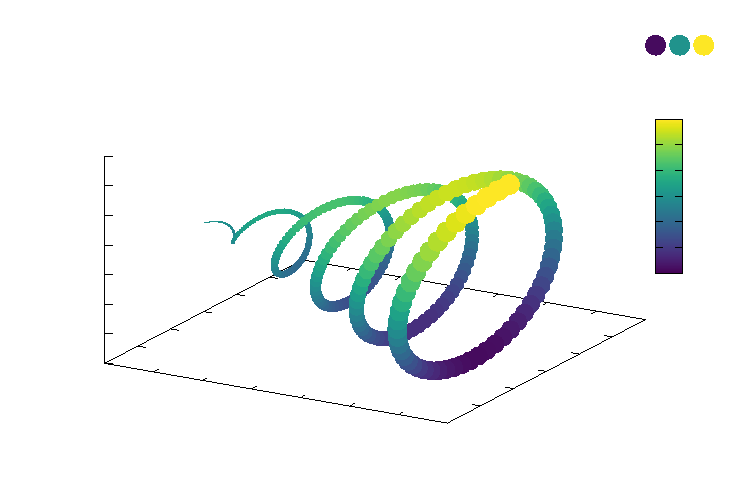
\includegraphics[width={360.00bp},height={237.00bp}]{test_line3d}}%
    \gplfronttext
  \end{picture}%
\endgroup
